%%%%%%%%%%%%%%%%%%%%%%%%%%%%%%%%%%%%%%%%%
% fphw Assignment
% LaTeX Template
% Version 1.0 (27/04/2019)
%
% This template originates from:
% https://www.LaTeXTemplates.com
%
% Authors:
% Class by Felipe Portales-Oliva (f.portales.oliva@gmail.com) with template 
% content and modifications by Vel (vel@LaTeXTemplates.com)
%
% Template (this file) License:
% CC BY-NC-SA 3.0 (http://creativecommons.org/licenses/by-nc-sa/3.0/)
%
%%%%%%%%%%%%%%%%%%%%%%%%%%%%%%%%%%%%%%%%%

%----------------------------------------------------------------------------------------
%	PACKAGES AND OTHER DOCUMENT CONFIGURATIONS
%----------------------------------------------------------------------------------------

\documentclass[
  french,
  % twocolumn,
	11pt, % Default font size, values between 10pt-12pt are allowed
	%letterpaper, % Uncomment for US letter paper size
	%spanish, % Uncomment for Spanish
]{fphw}

% \usepackage[fontsize=10.0]{scrextend} % Use this to force the fontsize

%% Commands for numbering paragraphs
\renewcommand\thesection{\Roman{section}}
\renewcommand\thesubsection{\thesection.\arabic{subsection}}
\renewcommand*\thesubsubsection{%
  \Roman{section}.\arabic{subsection}.\alph{subsubsection}%
}

% Template-specific packages
\usepackage{babel}
\usepackage[utf8]{inputenc} % Required for inputting international characters
% \usepackage{DejaVuSerifCondensed} 
\usepackage[T1]{fontenc} % Output font encoding for international characters

\usepackage{kpfonts}        %% For math only
\usepackage{fontspec}       %% Because we are using XeTEX
\setromanfont{Minion Pro}   %% For text (Minion Math is commercial)

%-----------------------------------------------------------------------
% \setromanfont{Meta Serif Pro}
% \setsansfont{Fira Sans}
% \setmonofont[Color={0019D4}]{Fira Code} 
%-----------------------------------------------------------------------

\usepackage{fancyvrb}
\usepackage{fvextra}
\newcommand\userinput[1]{\textbf{#1}}
\newcommand\arguments[1]{\textit{#1}}

\usepackage{amsmath}
\usepackage{mathtools}
\usepackage{xfrac} 

\usepackage{graphicx} % Required for including images
\usepackage[textfont=it,font=small]{caption}  %% To manage long captions in images
\usepackage{subcaption}
\captionsetup{justification=centering}

\usepackage{float}
\graphicspath{ {../img/} }

\usepackage{booktabs} % Required for better horizontal rules in tables

\usepackage{listings} % Required for insertion of code

\usepackage{array} % Required for spacing in tabular environment

\usepackage{enumerate} % To modify the enumerate environment

\usepackage{amssymb}
\usepackage{enumitem}	%% % To modify the itemize bullet character

\newcommand{\tabhead}[1]{{\bfseries#1}}

\usepackage{xcolor}
\usepackage{listings}
\colorlet{mygray}{black!30}
\colorlet{mygreen}{green!60!blue}
\colorlet{mymauve}{red!60!blue}
\lstset{
  backgroundcolor=\color{gray!10},  
  basicstyle=\ttfamily,
  columns=fullflexible,
  breakatwhitespace=false,      
  breaklines=true,                
  captionpos=b,                    
  commentstyle=\color{mygreen}, 
  extendedchars=true,              
  frame=single,                   
  keepspaces=true,             
  keywordstyle=\color{blue},      
  language=c++,                 
  numbers=none,                
  numbersep=5pt,                   
  numberstyle=\tiny\color{blue}, 
  rulecolor=\color{mygray},        
  showspaces=false,               
  showtabs=false,                 
  stepnumber=5,                  
  stringstyle=\color{mymauve},    
  tabsize=3,                      
  title=\lstname                
}

\usepackage[linkcolor=blue,colorlinks=true]{hyperref}
% \usepackage[colorlinks=true,urlcolor=blue]{hyperref}
\hypersetup{citecolor=blue}

\usepackage{cleveref}
\usepackage{siunitx}
\usepackage{bm}

\usepackage[backend=bibtex,style=alphabetic,maxnames=2,natbib=true]{biblatex} % Use the bibtex backend with the alphabetic citation style (compact APA-like)
% \usepackage[backend=bibtex,style=authoryear,maxnames=2,natbib=true]{biblatex} % Use the bibtex backend with the authoryear citation style (which resembles APA)
\addbibresource{../bib/bibliography.bib} % The filename of the bibliography
\usepackage[autostyle=true]{csquotes} % Required to generate language-dependent quotes in the bibliography 
% \renewcommand*{\bibfont}{\tiny} % Pour reduire la taille des references

\usepackage[useregional=numeric]{datetime2}
\usepackage[normalem]{ulem}

% %-------------------------------------------------------------------------------

\newcommand{\myvec}[3]{\begin{pmatrix} #1  \\ #2 \\ #3 \end{pmatrix}}   %% vecteur 3d
\newcommand{\mymat}[9]{\begin{pmatrix} #1 & #2 & #3 \\ #4 & #5 & #6 \\ #7 & #8 &#9 \end{pmatrix}}  %% Matrice 3*3

\renewcommand{\vector}[4]{\begin{pmatrix} #1  \\ #2 \\ #3 \\ #4 \end{pmatrix}}   %% vecteur 4d
% \newcommand{\mymatrix}[16]{\begin{pmatrix} #1 & #2 & #3 & #4 \\ #4 & #6 & #7 & #8 \\ #9 & #10 & #11 & #12 \\ #13 & #14 & #15 & #16 \end{pmatrix}}  %% Matrice 3*3

\newcommand{\hquad}{\hspace{0.5em}} %% Bew command for half quad
\newcommand*\diff{\mathop{}\!\mathrm{d}}
% \setlength\parindent{0pt}	%% To remove all indentations
\newcommand{\bvec}[1]{\bm{\mathrm{#1}}}  %% Use this to make vectors
\newcommand{\bmat}[1]{\bm{\mathsf{#1}}}   %% Use this to make tensors

%----------------------------------------------------------------------------------------
%	ASSIGNMENT INFORMATION
%----------------------------------------------------------------------------------------

\title{Compte rendu semaine \#4} % Assignment title
% \title{Difficultés rencontrées} % Assignment title

\author{Desmond Roussel Nzoyem} % Student name

\date{\DTMdisplaydate{2021}{2}{24}{-1} - \DTMdisplaydate{2021}{3}{2}{-1}} % Due date

\institute{Sorbonne Université \\ Laboratoire Jacques-Louis Lions} % Institute or school name

\class{Stage M2} % Course or class name

\professor{Pr. Stéphane Labbé} % Professor or teacher in charge of the assignment

%----------------------------------------------------------------------------------------

\begin{document}

\maketitle % Output the assignment title, created automatically using the information in the custom commands above

%----------------------------------------------------------------------------------------
%	ASSIGNMENT CONTENT - INTRO
%----------------------------------------------------------------------------------------


Cette semaine je continue la lecture de la thèse de D. Balasoiu \parencite{balasoiu2020halthesis}. Comme je l'ai mentionné dans le rapport de la semaine 3, la compréhension est particulièrement difficile. Et je pense qu'il est impératif que je comprenne le Chapitre 3 et ses démonstrations avant d'avancer avec les processus stochastiques. Pour l'instant je suis bloqué à la section 3.2.2, et j'ai besoin d'aide pour avancer.


%----------------------------------------------------------------------------------------
%	ASSIGNMENT CONTENT - SECTION 1
%----------------------------------------------------------------------------------------

\section{Tâches effectuées}

\begin{enumerate}
  \item Continuation de lecture du chapitre 3 de \parencite{balasoiu2020halthesis}.
  \item Lecture des annexes de la thèse.
  \item Relecture (rapide) des chapitres précédents. 
\end{enumerate}

%----------------------------------------------------------------------------------------
%	ASSIGNMENT CONTENT - SECTION 2
%----------------------------------------------------------------------------------------

\section{Difficultés rencontrées}

\textit{Toutes ces questions concernent la proposition 3.3.1 de \parencite[p.93]{balasoiu2020halthesis}.}

\begin{enumerate}
  \item \sout{Comment est orienté le vecteur $e_\nu$ ? Cette quantité apparait pour la première fois au niveau de la définition de l'énergie élastique de torsion \parencite[p.91]{balasoiu2020halthesis}.} 
  \item \sout{Pouvez-vous s'il vous plait m'éclairer sur le début de la démonstration de la proposition 3.3.1 \parencite[p.93]{balasoiu2020halthesis} ?}
  % \begin{figure}[H]
  %   \centering
  %   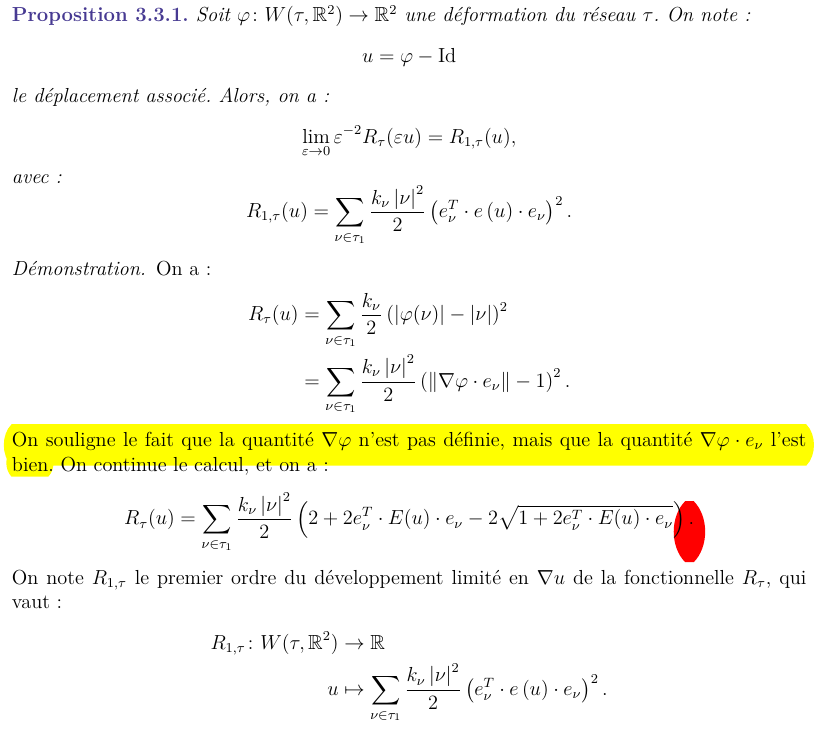
\includegraphics[width=0.7\textwidth]{Propo1.png}
  %   \caption{Difficulté à la proposition 3.3.1}
  % \end{figure}
  \item Je me suis rendu compte que je n'avais pas correctement lu la proposition 3.3.1.. En effet, c'est écrit "\textit{Soit $\varphi : W(\tau, \mathbb{R}^2) \rightarrow \mathbb{R}^2$} \ldots ". S'agit-il d'une erreur ? Puisque dans l'annexe B, l'ensemble de départ pour $\varphi$ est $\overline{\Omega}$.
  \item Toujours au tout début de la démonstration de la proposition 3.3.1, il me semble que l'égalité $$\vert \varphi (\nu) \vert = \vert \nu \vert \times \Vert \nabla \varphi \cdot e_{\nu} \Vert$$ a été utilisée (voir figure 1 ci-bas). Je ne comprends pas son origine.
  \begin{figure}[H]
    \centering
    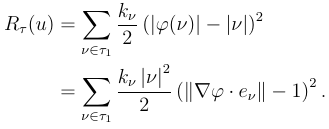
\includegraphics[width=0.4\textwidth]{Propo12.png}
    \caption{Début de démonstration de la proposition 3.3.1 \parencite[p.93]{balasoiu2020halthesis}.}
  \end{figure}
  % \textit{Pouvez-vous aussi confirmer que dans toute la thèse, quand on écrit juste $\nabla \varphi$, il s'agit en effet du gradient au point $\nu$, i.e. $\nabla \varphi(\nu)$?}
  \item Des simples $\vert \cdot \vert$ et des doubles $\Vert \cdot \Vert$ barres sont utilisées pour les normes. Conformément à votre réponse pour la question 2 ci-haut (mercredi), la quantité $\Vert \nabla \varphi \cdot e_{\nu} \Vert$ est un vecteur de $\mathbb{R}^2$, au même titre que $\nu$ ou $\varphi(\nu)$. Ne s'agit-il pas de la même norme ?
  \item Pouvez-vous confirmer que la notation $R_{1,\tau}$ pour le \textbf{premier} ordre du développement limité de $R_{\tau}$ ne désigne pas forcément l'ordre \textbf{1 (un)}? Et qu'il s'agit en fait du degré du monôme de plus faible degré dans le développement limité de $R_{\tau}$?
  \item Ensuite, \citeauthor{balasoiu2020halthesis} dit que la fonctionnelle $R_{1,tau}$ est \textbf{quadratique}. En regardant l'expression obtenue en fonction de $e(u)$, je peux voire le caractère quadratique en fonction de $\nabla u$, mais pas en fonction de $u$. En plus, je ne vois pas ce que cette assertion apporte à la démonstration, surtout que l'existence d'un développement en série entière pour $R_{2,\tau}$ repose sur l'hypothèse "\textit{$u$ suffisamment petit}", et donc $\lim_{k \to \infty} R_{2,\tau}(u) = 0$ i.e. (rayon de convergence non nul).
\end{enumerate}

%----------------------------------------------------------------------------------------
%	ASSIGNMENT CONTENT - SECTION 3
% ----------------------------------------------------------------------------------------

\section{Sujets explorables}

\begin{enumerate}
  \item 
\end{enumerate}

% %-------------------------------------------------------------------------------
% %							THE BIBLIOGRAPHY
% %-------------------------------------------------------------------------------
\clearpage   % Pour retirer les references de la bare de navigation
\printbibliography


\end{document}
